\documentclass[12pt,letterpaper]{report}

\usepackage{geometry}
\usepackage{graphicx}
\usepackage{longtable}
\usepackage{array}
\usepackage{verbatim}
\usepackage{hyperref}
\graphicspath{{report/assets/}{assets/}}

\geometry{margin=1in}
\linespread{1.25}

\hypersetup{
    colorlinks=true,
    linkcolor=blue,
    urlcolor=blue,
    citecolor=blue,
    pdftitle={AI SaaS Chatbot Project Report},
    pdfauthor={Student Name}
}

\newcommand{\screenshotplaceholder}[2]{
\begin{figure}[h]
\centering
\fbox{
\parbox[c][1.5in][c]{0.9\textwidth}{
\centering
\textbf{#1}\\[0.2cm]
#2\\[0.2cm]
\textit{(Insert screenshot after running the system)}
}
}
\caption{#1}
\end{figure}
}

\begin{document}

% ------------------ Title Page ------------------
\begin{titlepage}
    \centering
    {\Large PROJECT REPORT\par}
    \vspace{1.2cm}
    {\huge\bfseries AI SAAS CHATBOT USING RETRIEVAL-AUGMENTED GENERATION\par}
    \vspace{1.2cm}
    {\Large Submitted in partial fulfillment of the requirements\par}
    {\Large for the award of\par}
    \vspace{0.6cm}
    {\Large Bachelor of Engineering in Computer Engineering\par}
    \vspace{1.2cm}
    {\large by\par}
    \vspace{0.3cm}
    {\Large\bfseries Your Name Here\par}
    {\large Roll No: XXXX\par}
    \vspace{1.2cm}
    {\large Under the guidance of\par}
    {\Large\bfseries Prof. Guide Name\par}
    \vfill
    {\Large Department of Computer Engineering\par}
    {\Large College Name\par}
    {\Large University Name\par}
    \vspace{0.6cm}
    {\Large 2025--2026\par}
\end{titlepage}

% ------------------ Certificate ------------------
\chapter*{Certificate}
\addcontentsline{toc}{chapter}{Certificate}
This is to certify that the project report entitled \textbf{``AI SaaS Chatbot using Retrieval-Augmented Generation''} is a bonafide work carried out by \textbf{Your Name Here} under my supervision and guidance during the academic year 2025--2026, in partial fulfillment of the requirements for the award of the degree of Bachelor of Engineering in Computer Engineering.

\vspace{2cm}
\noindent Guide Signature: \hrulefill

\vspace{1cm}
\noindent Head of Department: \hrulefill

\vspace{1cm}
\noindent Principal: \hrulefill

\vspace{1cm}
\noindent Date: \hrulefill

\vspace{1cm}
\noindent Place: \hrulefill

% ------------------ Declaration ------------------
\chapter*{Declaration}
\addcontentsline{toc}{chapter}{Declaration}
I hereby declare that the project report entitled \textbf{``AI SaaS Chatbot using Retrieval-Augmented Generation''} is my own work carried out under the supervision of my guide. This report has not been submitted to any other university or institute for the award of any degree or diploma.

\vspace{2cm}
\noindent Student Signature: \hrulefill

\vspace{1cm}
\noindent Name: \hrulefill

\vspace{1cm}
\noindent Date: \hrulefill

% ------------------ Acknowledgement ------------------
\chapter*{Acknowledgement}
\addcontentsline{toc}{chapter}{Acknowledgement}
I express my sincere gratitude to my project guide and the faculty members of the Department of Computer Engineering for their guidance, timely support, and constructive feedback throughout this work. I also thank my classmates and family for their encouragement. Their input helped in converting an initial prototype into a structured, evaluated, and production-minded Retrieval-Augmented Generation (RAG) system.

% ------------------ Abstract ------------------
\chapter*{Abstract}
\addcontentsline{toc}{chapter}{Abstract}
This project presents the design and implementation of an AI SaaS chatbot backend using Retrieval-Augmented Generation (RAG). The objective is to provide accurate, context-grounded responses by combining semantic retrieval from enterprise documents with large language models (LLMs). The system supports multiple providers (Groq and Google Gemini), local embedding generation using Hugging Face embeddings, persistent vector storage through ChromaDB, and conversation memory through SQLite.

The architecture is designed for practical deployment and maintainability. It includes a structured ingestion pipeline for PDF, TXT, CSV, Excel, and JSON files; a retrieval layer with configurable chunking and top-k search; a generation layer with strict context-grounding prompts; and API endpoints implemented in FastAPI. To improve reliability, the system contains model fallback logic for quota limits and transient provider failures. To improve reproducibility and DevOps readiness, the project includes Docker containerization, automated data ingestion orchestration, observability hooks via LangSmith, and a quantitative RAG quality evaluation framework via Ragas.

A testing suite using Pytest validates ingestion behavior and core RAG flow. The result is a professional backend foundation that demonstrates the complete AI application lifecycle: data ingestion, indexing, retrieval, generation, observability, evaluation, and operational automation. The work highlights practical tradeoffs, current limitations, and a roadmap for enterprise hardening such as authentication, async ingestion queues, and hybrid retrieval with reranking.

\textbf{Keywords:} Retrieval-Augmented Generation, Machine Learning, Natural Language Processing, ChromaDB, LangChain, FastAPI, Ragas, LangSmith, MLOps.

% ------------------ TOC and lists ------------------
\pagenumbering{roman}
\tableofcontents
\listoffigures
\listoftables

\chapter*{List of Abbreviations}
\addcontentsline{toc}{chapter}{List of Abbreviations}
\begin{longtable}{p{0.25\textwidth}p{0.65\textwidth}}
\textbf{Abbreviation} & \textbf{Expansion} \\
\hline
AI & Artificial Intelligence \\
API & Application Programming Interface \\
CSV & Comma Separated Values \\
EDA & Exploratory Data Analysis \\
JSON & JavaScript Object Notation \\
LLM & Large Language Model \\
MLOps & Machine Learning Operations \\
NLP & Natural Language Processing \\
PDF & Portable Document Format \\
RAG & Retrieval-Augmented Generation \\
SaaS & Software as a Service \\
SQL & Structured Query Language \\
TXT & Plain Text File Format \\
UI & User Interface \\
\end{longtable}

\clearpage
\pagenumbering{arabic}

% ------------------ Chapter 1 ------------------
\chapter{Introduction}

\section{Overview}
The recent adoption of generative AI in SaaS products has changed expectations for customer support, internal search, onboarding, and knowledge management. End users now expect natural language interfaces that can answer complex questions from proprietary business documents. Standard LLM chat interfaces, however, are often not sufficient for enterprise usage because they can hallucinate and lack direct access to current domain data. 

Retrieval-Augmented Generation (RAG) addresses this by attaching a retrieval stage before generation. Instead of asking the model to answer from its internal pretraining alone, the system retrieves relevant chunks from a curated document store and injects them into the prompt context. This approach improves factual grounding and reduces unsupported claims. 

The project implemented in this report is an AI SaaS chatbot backend based on this RAG principle. The system is engineered with practical deployment goals: support for multiple LLM providers, local vector persistence, reproducible ingestion, memory across multi-turn conversations, error handling, and quantitative evaluation. The implementation is designed to operate as a realistic backend service rather than as an isolated notebook experiment.

\section{Machine Learning Context}
Machine learning is the computational framework that allows systems to discover patterns from data and make predictions or decisions with minimal explicit rule coding. In chatbot systems, machine learning appears in multiple layers:
\begin{itemize}
\item Embedding models convert text into dense vectors capturing semantic meaning.
\item Retrieval models rank stored chunks by vector similarity.
\item Generative LLMs synthesize responses conditioned on retrieved evidence.
\item Evaluation models score response quality using objective metrics.
\end{itemize}

Traditional software can match keywords, but ML-driven semantic encoding allows conceptual matching, where user intent and retrieved content can align even when exact words differ. In this project, a Hugging Face embedding model is used to create vector representations and ChromaDB stores and indexes those vectors for fast similarity lookup.

\section{Machine Learning Strategies Relevant to This Work}
\subsection{Supervised Learning}
Supervised learning uses labeled data to learn mappings from input to output. In the context of this project, supervised logic appears indirectly in pretrained embeddings and LLMs that were trained on massive supervised and instruction-tuned corpora. Although this project does not train an LLM from scratch, it deploys supervised-learning products as inference components.

\subsection{Unsupervised and Self-Supervised Learning}
Unsupervised and self-supervised paradigms underpin representation learning for text embeddings. The system benefits from this through pretrained embeddings that encode semantic relationships without requiring task-specific labels from the project team.

\subsection{Reinforcement and Preference Optimization (Background)}
Modern LLM behavior is often shaped by reinforcement learning from human feedback or preference optimization methods. This report includes this topic as background because the deployed providers (Gemini and Groq-hosted open models) include alignment behavior from such training. This matters for practical chatbot performance, safety, and tone.

\section{Problem Statement}
Organizations often maintain support content in fragmented formats: PDF manuals, CSV exports, spreadsheets, and internal notes. Users ask questions in natural language, but static search interfaces return weak results, while direct LLM chats may return ungrounded answers. 

The project aims to solve this gap by building a retrieval-grounded chatbot backend that can:
\begin{itemize}
\item ingest multi-format documents,
\item index and retrieve context semantically,
\item generate concise and context-bounded answers,
\item preserve conversational continuity with memory,
\item remain observable and testable in production-like workflows.
\end{itemize}

\section{Objectives}
The principal objectives are:
\begin{enumerate}
\item Build a robust ingestion pipeline for common enterprise document formats.
\item Create a persistent local vector database for semantic retrieval.
\item Implement a multi-provider LLM layer with fallback behavior.
\item Expose the full pipeline through a FastAPI interface.
\item Add reproducibility through Docker, testing, and operational scripts.
\item Add quality and observability frameworks using Ragas and LangSmith.
\end{enumerate}

\section{Scope and Deliverables}
The project scope includes backend design and implementation of the RAG system and core MLOps capabilities. Frontend work exists as a separate React artifact but is not the primary focus of this report. The final deliverables are source code modules, configuration files, technical documentation, automated tests, and this formal project report.

\section{Report Organization}
The remaining chapters are organized as follows:
\begin{itemize}
\item Chapter 2 reviews related literature and industrial patterns in RAG systems.
\item Chapter 3 details methodology, architecture, algorithms, and module design.
\item Chapter 4 explains implementation, testing, results, and discussion.
\item Chapter 5 presents conclusions and future enhancements.
\item Appendices include representative source code and supporting artifacts.
\end{itemize}

% ------------------ Chapter 2 ------------------
\chapter{Literature Survey}

\section{Related Work in Retrieval-Augmented Generation}
RAG emerged as a practical bridge between parametric memory (inside LLM weights) and non-parametric memory (external documents). Earlier question-answering systems used sparse lexical retrieval and template-based response logic. With transformer-based embeddings, dense retrieval became dominant for semantic search use cases. Recent SaaS products combine dense retrieval with LLM generation to provide support copilots, internal assistants, and domain-specific chat interfaces.

The key insight from literature is that generation quality depends strongly on retrieval quality. Even a strong LLM performs poorly when irrelevant or incomplete context is retrieved. Therefore, robust systems focus on data chunking, metadata tracking, retriever configuration, and evaluation metrics.

\section{Document Ingestion and Chunking Strategies}
A recurring theme in research and engineering practice is chunking strategy. Very small chunks may lose semantic continuity; very large chunks can exceed token budgets and reduce retriever precision. Recursive splitters that prioritize paragraph and sentence boundaries typically outperform naive fixed-character segmentation in readability and grounding fidelity.

This project adopts RecursiveCharacterTextSplitter with configurable chunk size and overlap. This allows balancing retrieval granularity against context cohesion.

\section{Vector Databases for Semantic Retrieval}
Vector databases such as ChromaDB, Qdrant, Weaviate, and Pinecone are now standard components in RAG stacks. They support indexing and nearest-neighbor lookup over high-dimensional embeddings. Local embedded vector stores are useful in early-stage development due to simplicity, while managed or distributed stores are preferred in high-scale enterprise deployment.

The present implementation uses ChromaDB in persistent local mode. This is appropriate for educational and prototype-to-SME deployments and supports reproducibility in offline development.

\section{LLM Provider Strategy and Reliability}
Production systems increasingly avoid hard dependence on one provider. Service outages, quota limits, and model lifecycle changes can disrupt user-facing chatbot operations. A common strategy is primary-plus-fallback model routing. Error categorization (quota, unavailable model, transient upstream error) is critical for deciding whether to retry, fail fast, or switch models.

The system described in this report includes explicit model fallback sequencing and provider-agnostic exception handling. This design follows resilient service principles from modern AI operations.

\section{Observability and Evaluation Practices}
A major weakness in many student and startup RAG systems is lack of observability. Without trace-level visibility, debugging poor responses is difficult. Platforms such as LangSmith provide retrieval traces, prompts, and output chains for root-cause analysis.

Similarly, objective evaluation frameworks are essential. Ragas provides measurable metrics such as faithfulness, answer relevancy, context precision, and context recall. Literature shows that such metrics enable controlled iteration and regression detection.

\section{Testing and MLOps Lifecycle}
Classic ML pipelines were often evaluated offline and deployed with limited integration testing. Current MLOps standards emphasize continuous validation: data ingestion checks, unit tests, behavior regressions, and deployment reproducibility. Containerization, infrastructure automation, and CI hooks convert research prototypes into operational systems.

This project aligns with that direction by combining backend modules, tests, documentation, Docker deployment files, and operational automation scripts.

\section{Research Gaps and Relevance to This Project}
Key gaps identified across related work include:
\begin{itemize}
\item limited grounding controls in naive chatbot implementations,
\item insufficient operational reliability under provider failures,
\item missing quality baselines and poor experiment traceability,
\item lack of ingestion automation for frequently updated corpora.
\end{itemize}

The implemented system addresses these gaps with explicit prompt constraints, model fallback, evaluation and tracing support, and ingestion orchestration. While not yet a fully hardened global-scale architecture, it represents a comprehensive, production-minded educational implementation.

% ------------------ Chapter 3 ------------------
\chapter{Methodology and System Design}

\section{Existing System}
The baseline problem pattern observed in many early chatbot projects includes:
\begin{itemize}
\item one-time manual ingestion,
\item ad hoc scripts without persistent memory,
\item no fallback for LLM failures,
\item limited or absent quality metrics,
\item weak deployment reproducibility.
\end{itemize}

Such systems may work during demonstrations but fail under realistic usage where document sets evolve, model APIs face limits, and multi-turn context matters.

\section{Proposed System}
The proposed architecture is a layered RAG backend with the following modules:
\begin{enumerate}
\item \textbf{Ingestion Layer}: Loads PDF, TXT, CSV, XLSX, and JSON sources.
\item \textbf{Chunking Layer}: Applies recursive splitting with overlap.
\item \textbf{Embedding and Indexing Layer}: Generates vectors and persists in ChromaDB.
\item \textbf{Retrieval Layer}: Fetches top-k semantically relevant chunks.
\item \textbf{Generation Layer}: Uses provider-selected LLM with fallback sequence.
\item \textbf{Memory Layer}: Stores chat history in SQLite by chat\_id.
\item \textbf{API Layer}: Exposes endpoints for health and question-answer flow.
\item \textbf{Operations Layer}: Adds Docker, observability, evaluation, and automation.
\end{enumerate}

\section{Functional Requirements}
\begin{itemize}
\item Ingest heterogeneous document formats.
\item Build and persist vector embeddings.
\item Retrieve relevant context for user queries.
\item Generate concise responses grounded in retrieved data.
\item Support multi-turn conversation memory.
\item Provide API endpoints for external clients.
\item Expose diagnostic behavior for failures.
\end{itemize}

\section{Non-Functional Requirements}
\begin{itemize}
\item Maintainability through modular Python files.
\item Extensibility for additional providers and retrievers.
\item Reliability via retry/fallback behavior.
\item Reproducibility via Dockerized environment.
\item Observability via traces and evaluation metrics.
\end{itemize}

\section{Software and Hardware Requirements}
\subsection{Software Requirements}
\begin{itemize}
\item Python 3.11
\item FastAPI, Uvicorn
\item LangChain ecosystem modules
\item ChromaDB
\item Hugging Face embedding dependencies
\item Pytest for testing
\item Docker and Docker Compose
\end{itemize}

\subsection{Hardware Requirements}
\begin{itemize}
\item Minimum 8 GB RAM (16 GB recommended for smooth local model operations)
\item Multi-core CPU
\item SSD storage for vector index and local data
\item Stable internet for cloud LLM providers
\end{itemize}

\subsection{Core Libraries Used}
\begin{table}[h]
\centering
\begin{tabular}{p{0.32\textwidth}p{0.55\textwidth}}
\hline
\textbf{Library} & \textbf{Purpose} \\
\hline
langchain / langchain-core & Prompt chaining and retrieval pipeline orchestration \\
langchain-groq & Groq LLM integration \\
langchain-google-genai & Gemini model and embedding integrations \\
langchain-chroma & Vector store connection \\
pydantic-settings & Configuration management from environment variables \\
fastapi & HTTP API framework \\
sqlite3 & Persistent local chat memory \\
ragas & RAG quality evaluation metrics \\
watchdog & File watching for automated ingestion \\
pytest & Automated test execution \\
\hline
\end{tabular}
\caption{Major software dependencies in the project.}
\end{table}

\section{Programming Language Rationale}
Python was selected because it offers mature libraries for NLP, rapid API development, and MLOps tooling. Its ecosystem includes direct support for RAG components and easy integration with vector stores, LLM providers, and testing frameworks.

\section{System Architecture}
\subsection{Logical Architecture View}
The platform is intentionally separated into operational layers so each engineering concern remains independently maintainable. The presentation layer handles user interaction and request initiation. The API layer enforces schema validation and HTTP contracts. The orchestration layer handles retrieval logic, prompt assembly, and fallback decisions. The knowledge layer is responsible for vector retrieval and conversational state persistence. DataOps automates ingestion and corpus refresh, while the MLOps layer provides reproducibility, observability, and quality governance.

This layered split is not cosmetic. It creates explicit isolation boundaries between data movement, model inference, and platform reliability. That allows independent hardening of each subsystem and reduces blast radius during failures. For example, ingestion failures should not crash serving traffic, and model quota failures should trigger controlled fallback rather than unstructured API errors.

\begin{figure}[ht]
\centering
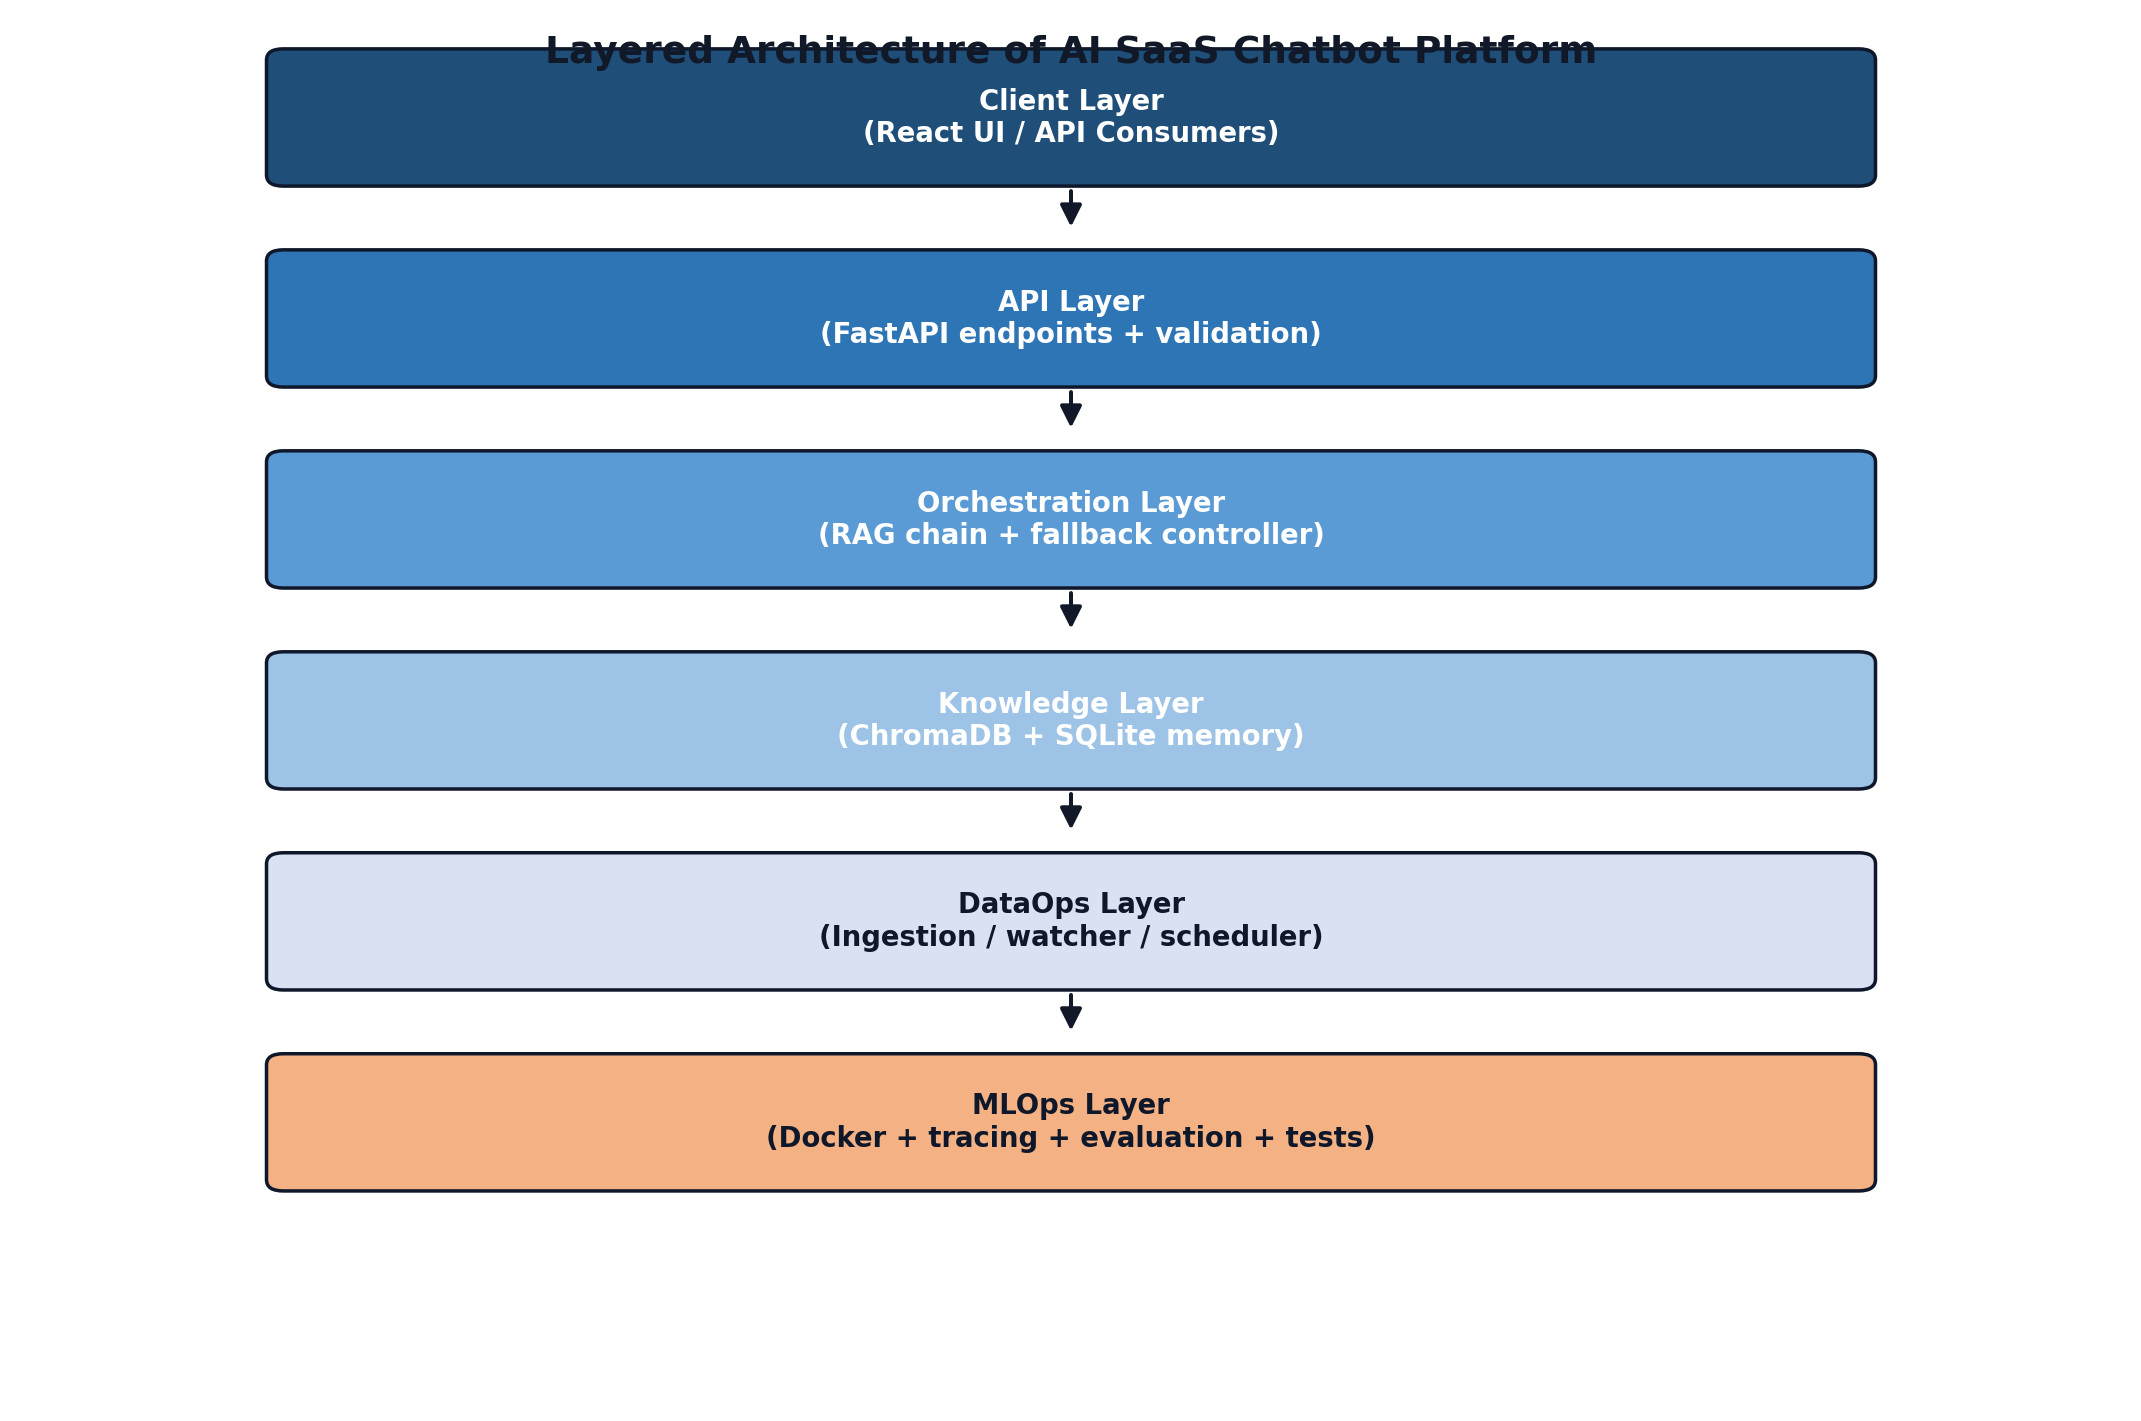
\includegraphics[width=0.97\textwidth]{architecture_layers.png}
\caption{Layered architecture used by the AI SaaS chatbot platform.}
\end{figure}

\subsection{Request-Response Runtime Sequence}
At runtime, each user query is processed through a deterministic sequence. Memory is loaded first to preserve multi-turn context. Retrieval then uses both the current question and recent conversational turns to disambiguate follow-up prompts. The generation payload is constructed only after retrieval, ensuring context-bounded outputs. The error path is explicitly classified, so only retryable conditions trigger fallback models. Finally, response metadata and messages are persisted for continuity and auditing.

This runtime sequence forms the primary control path of the application and is the core unit of production reliability. Any regression in this sequence directly affects correctness, latency, and user trust. For that reason, the flow is instrumented and designed to be observable and testable.

\begin{figure}[ht]
\centering
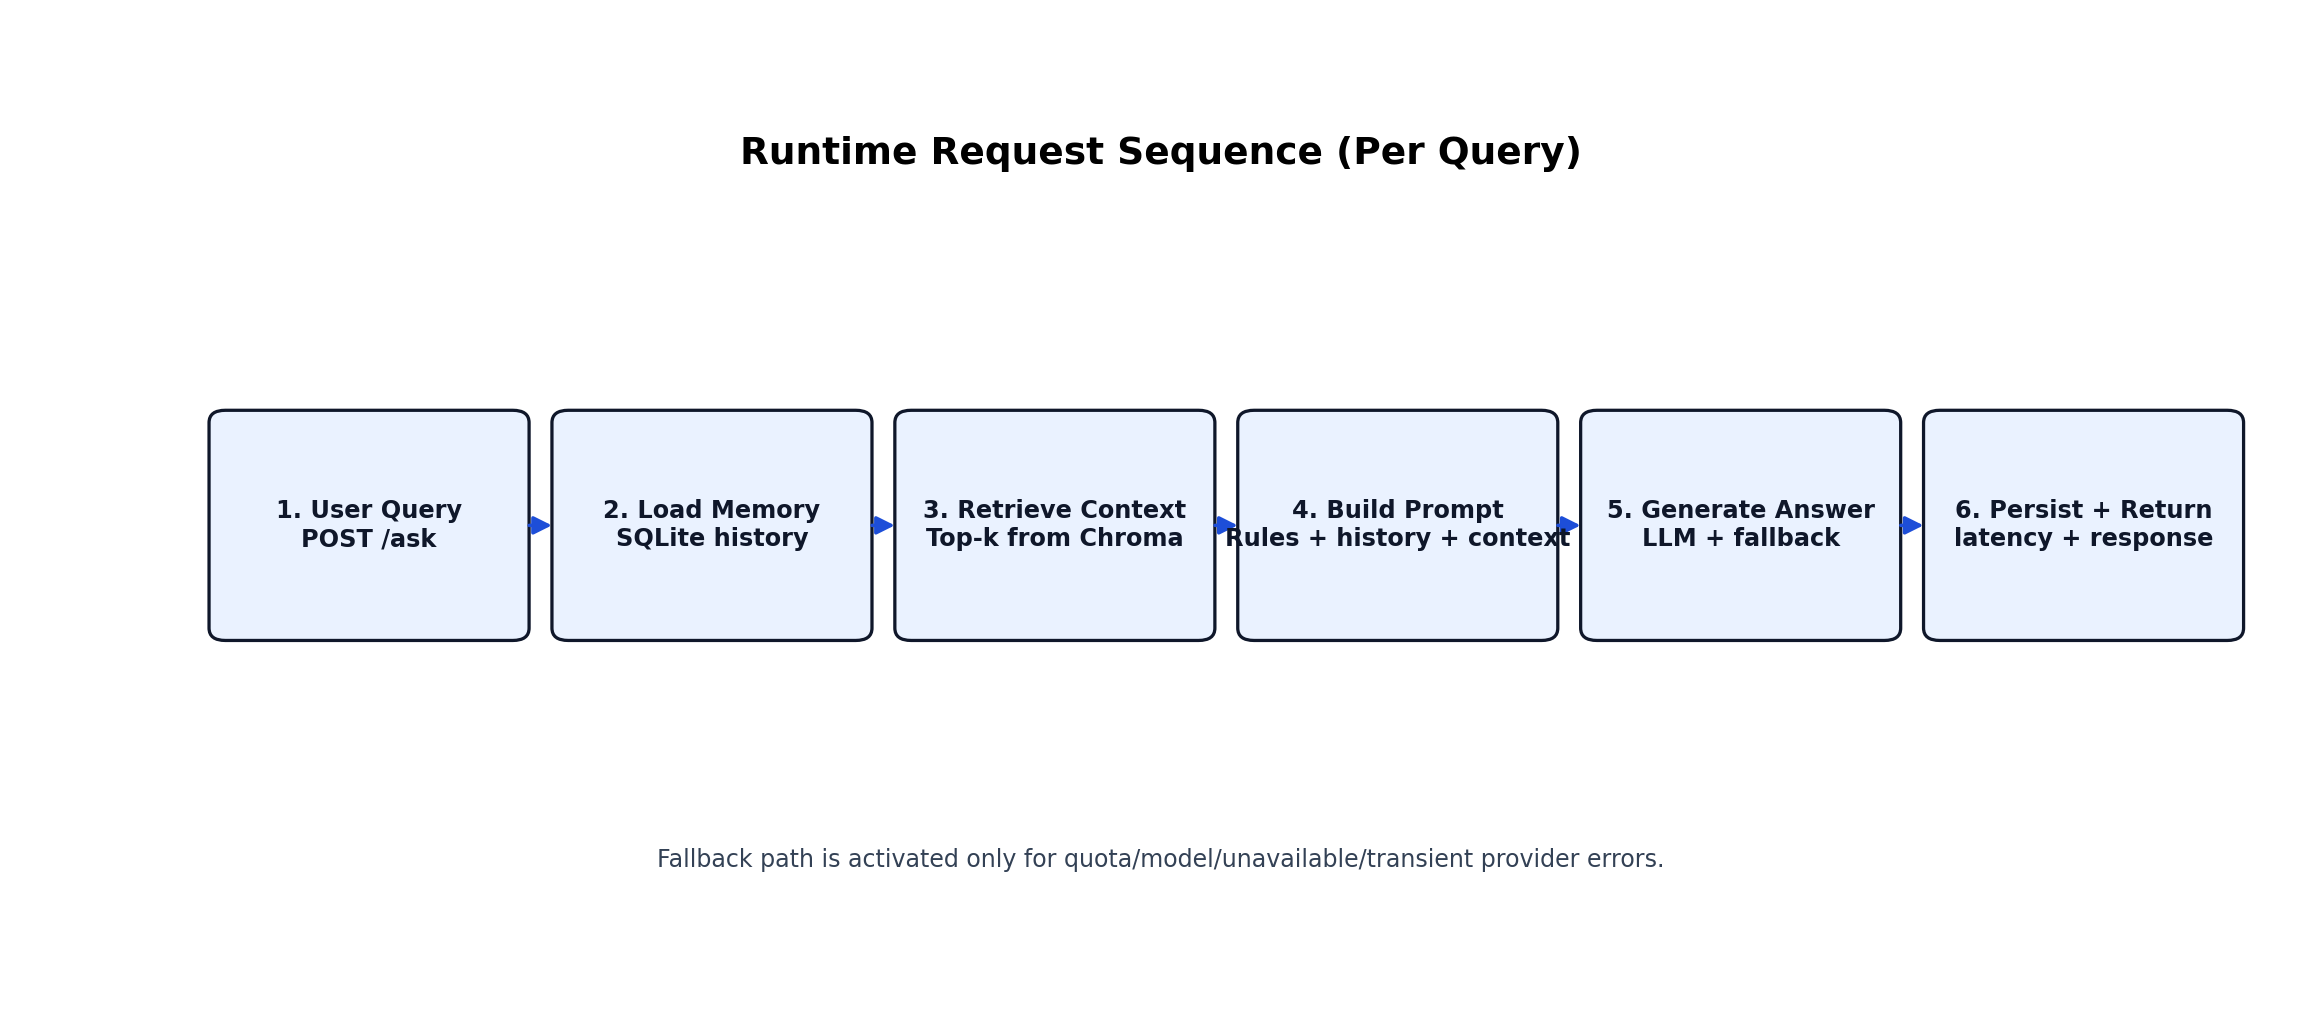
\includegraphics[width=0.98\textwidth]{runtime_sequence.png}
\caption{End-to-end runtime sequence for one production query.}
\end{figure}

\subsection{Deployment Architecture with Docker}
The deployment is container-centric and isolates API and vector database responsibilities:
\begin{itemize}
\item \textbf{api container}: Runs FastAPI/Uvicorn, RAG orchestration, retrieval logic, and memory interactions.
\item \textbf{chroma container}: Runs the vector database service with persistence enabled.
\item \textbf{bridge network}: Internal service-to-service communication using service names.
\item \textbf{health checks}: Container-level checks ensure service readiness before traffic.
\item \textbf{volumes}: Persistent mounts for \texttt{chroma\_db}, \texttt{data}, and \texttt{chat\_memory.db}.
\end{itemize}

The deployment topology is designed around two core services with explicit contracts: an API compute service and a vector database service. Network-level isolation keeps service communication private to the compose network, while mounted volumes preserve durable state across container restarts. This model makes local development and production-like validation behaviorally consistent.

\begin{figure}[ht]
\centering
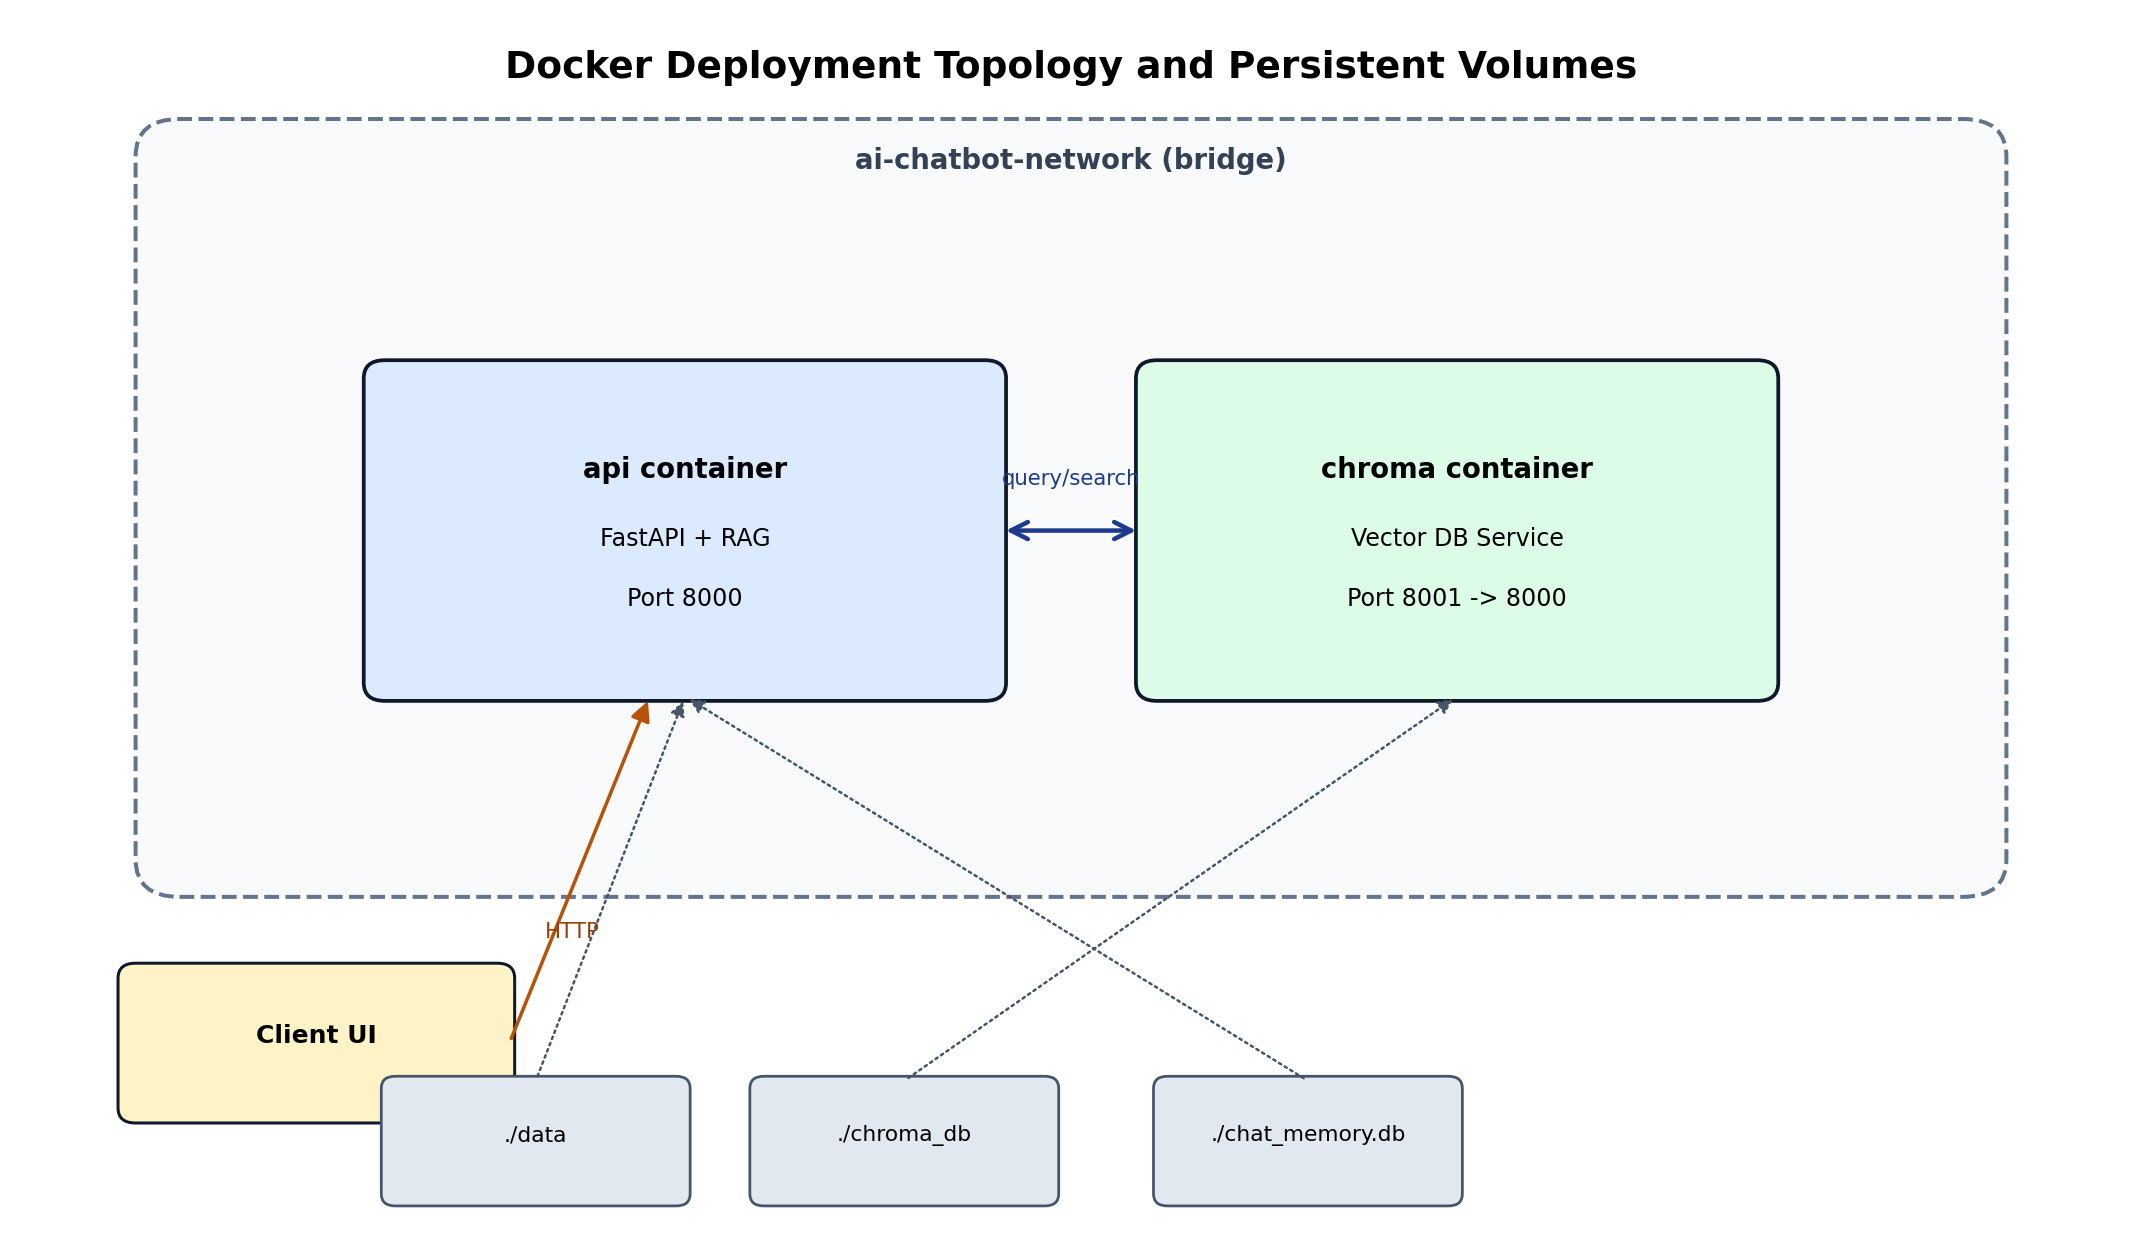
\includegraphics[width=0.97\textwidth]{docker_topology.png}
\caption{Container deployment topology from \texttt{docker-compose.yml}.}
\end{figure}

\subsection{Repository and Filesystem Architecture}
\begin{verbatim}
AI_SAAS(ChatBot) copy/
+-- backend/                    # Core platform modules
|   +-- api.py                  # FastAPI interface
|   +-- rag_engine.py           # Retrieval + generation orchestration
|   +-- ingest.py               # Multi-format ingestion and chunking
|   +-- vector_store.py         # ChromaDB integration
|   +-- memory.py               # SQLite persistent chat history
|   +-- evaluation.py           # Ragas quality evaluation
|   +-- observability.py        # LangSmith tracing integration
|   +-- file_watcher.py         # Event-based ingestion automation
|   +-- ingest_orchestrator.py  # watch/once/schedule/daemon modes
+-- frontend/                   # React frontend client
+-- data/                       # Ingestion source corpus
+-- docs/                       # Design, testing, MLOps documentation
+-- tests/                      # Pytest validation suite
+-- Dockerfile                  # Multi-stage Python image build
+-- docker-compose.yml          # API + Chroma service orchestration
+-- report/                     # Project report source and PDF
\end{verbatim}

\subsection{Data Representation Model}
\textbf{(A) Source corpus representation in this repository:}
\begin{table}[h]
\centering
\begin{tabular}{p{0.23\textwidth}p{0.16\textwidth}p{0.16\textwidth}p{0.3\textwidth}}
\hline
\textbf{File} & \textbf{Type} & \textbf{Size (bytes)} & \textbf{Role in Pipeline} \\
\hline
\texttt{product\_faq.txt} & TXT & 5339 & Domain knowledge source for semantic chunks \\
\texttt{golden\_dataset.json} & JSON & 3210 & Evaluation/benchmark question set \\
\texttt{test.csv} & CSV & 53 & Tabular ingestion validation sample \\
\hline
\end{tabular}
\caption{Current data assets in the \texttt{data/} directory.}
\end{table}

\textbf{(B) Internal metadata representation per document chunk:}
\begin{table}[h]
\centering
\begin{tabular}{p{0.24\textwidth}p{0.2\textwidth}p{0.45\textwidth}}
\hline
\textbf{Field} & \textbf{Type} & \textbf{Meaning} \\
\hline
\texttt{page\_content} & string & Raw text payload used for embedding and prompt context \\
\texttt{source} & string & Absolute or relative source file path \\
\texttt{row} & integer & Row index when data comes from CSV/XLSX records \\
\texttt{item} & integer & Item index when data comes from JSON arrays \\
\hline
\end{tabular}
\caption{Document metadata schema used for traceability and debugging.}
\end{table}

\textbf{(C) Retrieval and generation control representation:}
\begin{table}[h]
\centering
\begin{tabular}{p{0.34\textwidth}p{0.2\textwidth}p{0.34\textwidth}}
\hline
\textbf{Control Parameter} & \textbf{Current Value} & \textbf{Operational Impact} \\
\hline
\texttt{chunk\_size} & 500 & Controls retrieval granularity and context density \\
\texttt{chunk\_overlap} & 50 & Preserves continuity across adjacent chunks \\
\texttt{top\_k} & 4 & Number of retrieved chunks per query \\
\texttt{temperature} & 0.1 & Low-variance, factual response style \\
\texttt{memory\_max\_messages} & 6 & Limits history depth for prompt efficiency \\
\hline
\end{tabular}
\caption{Core retrieval/generation controls from runtime configuration.}
\end{table}

\subsection{Industrial Complexity in the Implemented System}
The complexity of this project is concentrated in integration and operations rather than a single algorithm:
\begin{enumerate}
\item \textbf{Provider abstraction with fallback}: supports multiple model backends and retry routing based on error classification.
\item \textbf{Context-grounded response enforcement}: system prompt constraints plus retrieval-driven answer policy reduce unsupported outputs.
\item \textbf{Stateful conversational memory}: persistent SQL-backed history with bounded replay for follow-up resolution.
\item \textbf{DataOps automation}: watcher and scheduler modes enable continuous corpus refresh without manual CLI intervention.
\item \textbf{Reproducible deployment}: multi-container orchestration with health checks and shared persistent volumes.
\item \textbf{Observability and measurable quality}: LangSmith traces and Ragas metrics provide diagnosable, testable model behavior.
\item \textbf{Failure-domain handling}: explicit API error mapping for quota, model availability, and upstream provider failures.
\end{enumerate}

The practical difficulty of this system lies in coordinating multiple failure-prone subsystems under one user-facing SLA: document pipelines, vector retrieval, model providers, state persistence, and HTTP serving. In production-like behavior, these components do not fail symmetrically. A model endpoint can rate-limit while ingestion is healthy; retrieval can succeed while answer generation fails; API uptime can remain high while answer quality drifts. A serious implementation must account for these mixed-mode states and preserve graceful degradation.

For this reason, the platform is treated as an iterative operations loop rather than a one-time model deployment. Each release cycle includes ingestion validation, retrieval verification, latency checks, trace inspection, and evaluation score review before promotion. This lifecycle orientation is the reason the project incorporates automation, monitoring, and quality measurement directly into the repository rather than as post-development add-ons.

\subsection{MLOps Lifecycle Diagram}
\begin{figure}[ht]
\centering
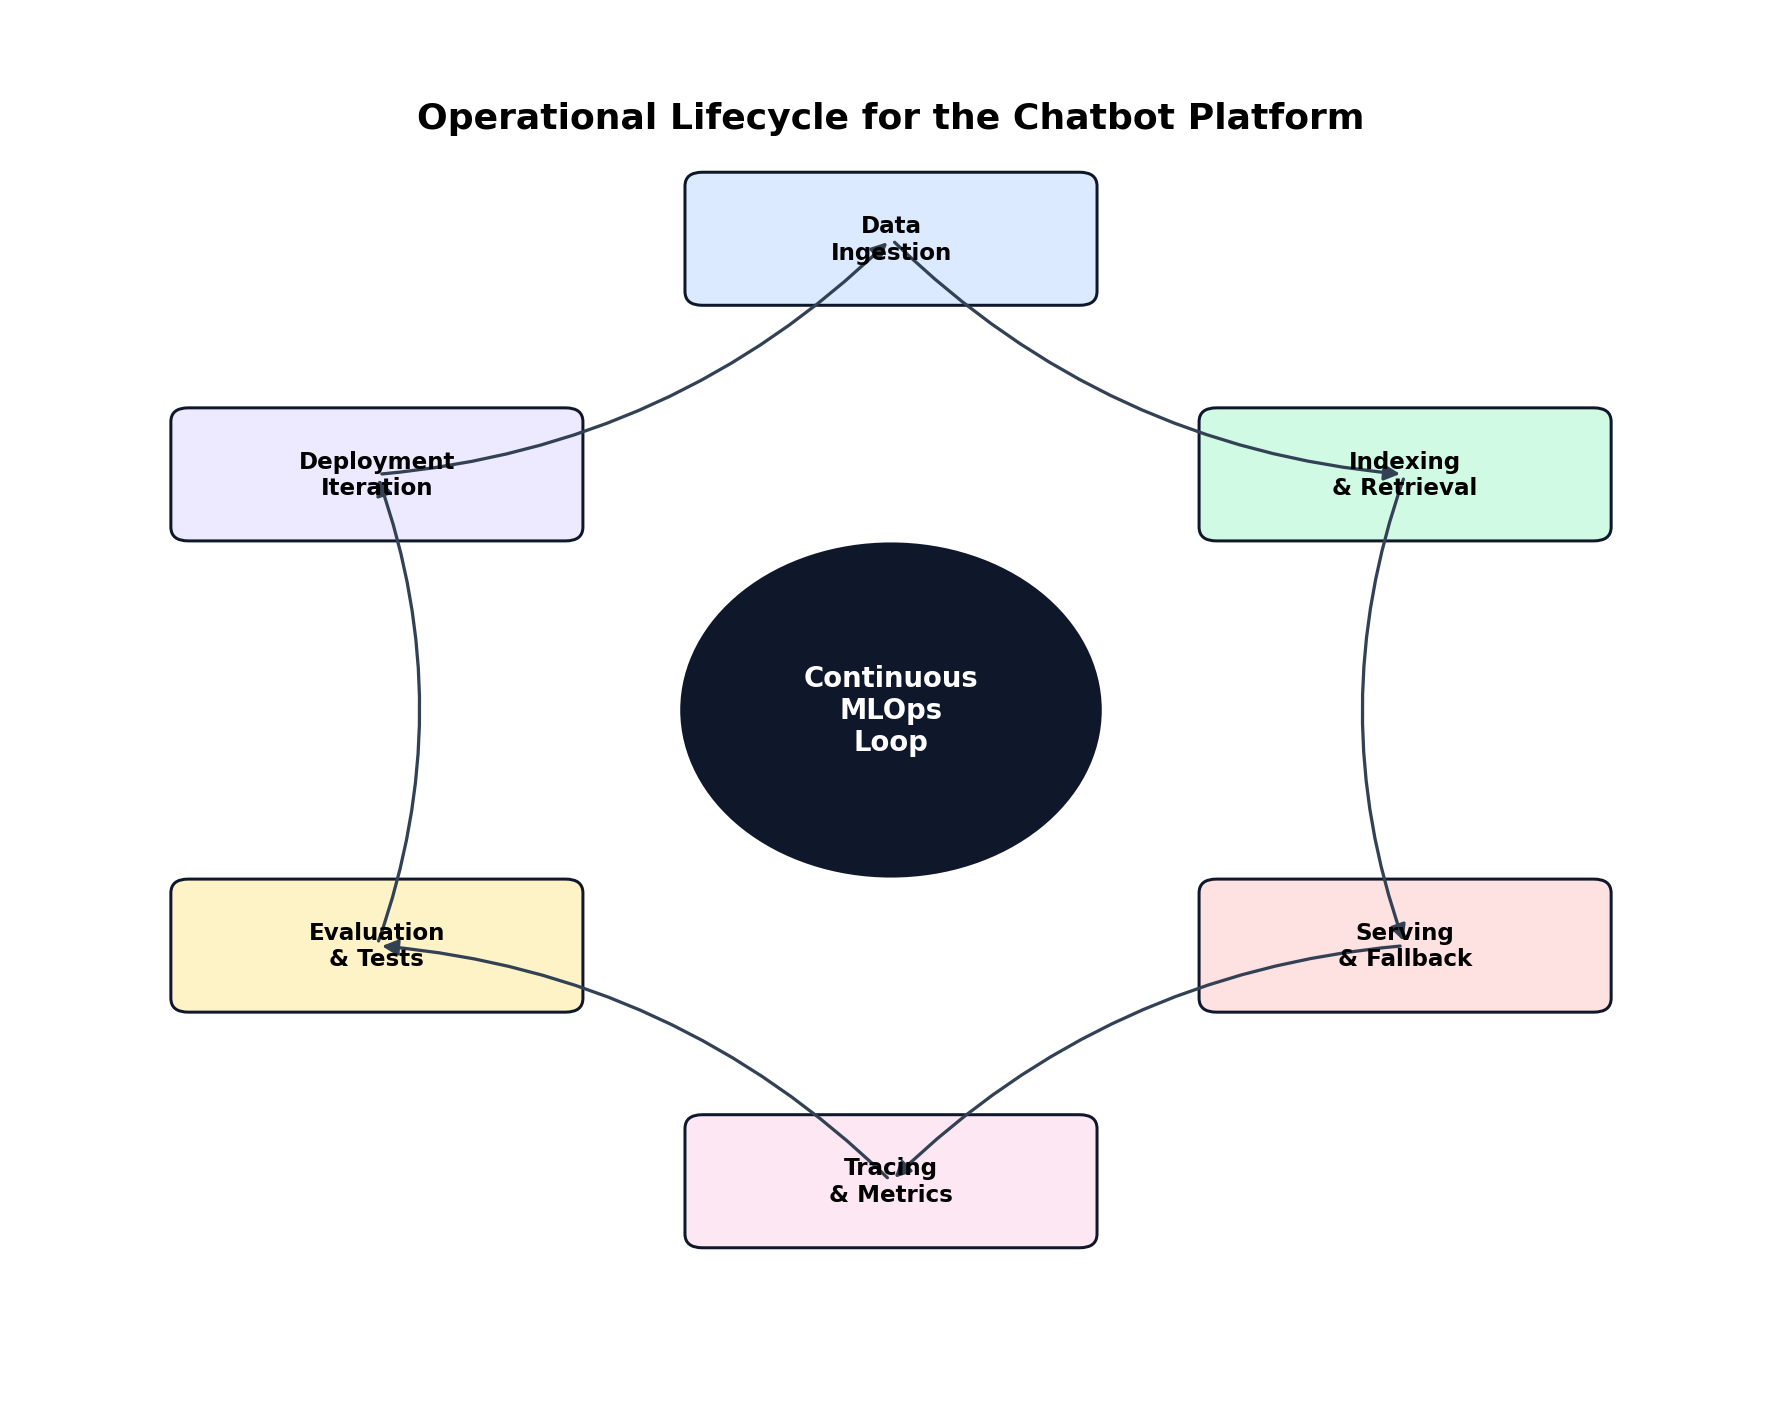
\includegraphics[width=0.82\textwidth]{mlops_lifecycle.png}
\caption{Continuous MLOps lifecycle used to operate and improve the platform.}
\end{figure}

The lifecycle in Figure above captures the operating principle used in this project: data ingestion feeds indexing; indexing feeds retrieval and serving; serving generates traces and quality metrics; metrics drive deployment and configuration iteration; iteration loops back into data and retrieval improvements. This closed-loop model is essential for RAG systems because data and user behavior evolve continuously even when application code remains unchanged.

\section{Algorithmic Flow}
\subsection{Data Ingestion Algorithm}
\begin{enumerate}
\item Scan target directory for supported extensions.
\item Load files through format-specific loaders.
\item Convert rows/items to documents with metadata.
\item Split into overlapping chunks recursively.
\item Push chunks to vector store with embeddings.
\end{enumerate}

\subsection{Retrieval and Generation Algorithm}
\begin{enumerate}
\item Accept user question and optional chat history.
\item Build retrieval query using recent conversation turns.
\item Retrieve top-k chunks from ChromaDB.
\item Create prompt with system rules, history, and context.
\item Invoke primary model.
\item If error is retryable (quota/unavailable/transient), attempt fallback model.
\item Return generated response or mapped API error.
\end{enumerate}

\subsection{Memory Management Algorithm}
\begin{enumerate}
\item Receive chat\_id with user request.
\item Read recent messages from SQLite table.
\item Pass messages into prompt as history placeholder.
\item After answer generation, append user and assistant messages.
\item Enforce configured history limits for retrieval and generation payload size.
\end{enumerate}

\section{Module-Wise Design}
\subsection{Configuration Module}
\texttt{backend/config.py} centralizes environment-driven settings such as provider, model names, fallback models, chunk size, top-k retrieval, temperature, and memory path.

\subsection{Ingestion Module}
\texttt{backend/ingest.py} handles multi-format data loading and recursive chunking. It supports PDF, TXT, CSV, Excel, and JSON input formats.

\subsection{Vector Store Module}
\texttt{backend/vector\_store.py} provides functions to create/load ChromaDB instances and ingest chunks with consistent embedding configuration.

\subsection{RAG Engine Module}
\texttt{backend/rag\_engine.py} composes retrieval, prompting, model invocation, fallback logic, and domain-level exception mapping.

\subsection{API Module}
\texttt{backend/api.py} exposes \texttt{/} health and \texttt{/ask} chatbot endpoints. It includes CORS policy, startup pre-warm, validation, and structured error responses.

\subsection{Memory Module}
\texttt{backend/memory.py} manages SQLite-based chat memory with indexed lookup by \texttt{chat\_id} and ordered replay for prompt history.

\subsection{Evaluation Module}
\texttt{backend/evaluation.py} integrates Ragas metrics to evaluate faithfulness, relevancy, context precision, and context recall.

\subsection{Observability Module}
\texttt{backend/observability.py} enables LangSmith tracing when API credentials are configured.

\subsection{Automation Modules}
\texttt{backend/file\_watcher.py} and \texttt{backend/ingest\_orchestrator.py} provide continuous/scheduled ingestion patterns.

\section{Design Decisions and Tradeoffs}
\begin{itemize}
\item \textbf{Local embeddings over cloud embeddings by default}: lower cost and offline-friendly, with slightly lower quality in some domains.
\item \textbf{Chroma local persistence}: simple and reproducible, but not ideal for distributed multi-instance scale.
\item \textbf{Prompt-grounded output rule}: reduces hallucination risk, may occasionally return insufficient-answer responses.
\item \textbf{Fallback across model candidates}: improves availability, but can create response style variance.
\end{itemize}

% ------------------ Chapter 4 ------------------
\chapter{Implementation, Results, and Discussion}

\section{Implementation Workflow and MLOps Staging}
Implementation was treated as a platform engineering process, not a one-pass coding exercise. Each module was developed with explicit integration contracts so behavior could be validated incrementally under realistic runtime conditions. This approach reduced late-stage coupling risk and made root-cause identification practical when failures appeared across data, retrieval, or provider boundaries.

The staging model below reflects how work was sequenced in practice: data pipeline stabilization first, then retrieval/generation orchestration, then reliability controls, and finally observability and evaluation loops. This order matters because later stages depend on confidence in upstream data and retrieval behavior.

Implementation followed an engineering lifecycle that maps to practical MLOps phases:
\begin{table}[h]
\centering
\begin{tabular}{p{0.16\textwidth}p{0.28\textwidth}p{0.45\textwidth}}
\hline
\textbf{Phase} & \textbf{Primary Components} & \textbf{Engineering Outcome} \\
\hline
DataOps & \texttt{ingest.py}, \texttt{file\_watcher.py}, \texttt{ingest\_orchestrator.py} & Automated multi-format ingestion and refresh pipeline \\
ModelOps & \texttt{embedder.py}, \texttt{vector\_store.py}, \texttt{rag\_engine.py} & Retrieval-grounded generation with model fallback control \\
ServingOps & \texttt{api.py}, \texttt{memory.py} & Stateful API surface for low-latency chat operations \\
ReliabilityOps & fallback logic, mapped exceptions, startup pre-warm & Controlled failure domains and lower cold-start latency \\
ObservabilityOps & \texttt{observability.py}, tracing configuration & Trace-level visibility of retrieval and generation path \\
EvaluationOps & \texttt{evaluation.py}, golden dataset support & Quantitative RAG quality baseline and regression framework \\
PlatformOps & Dockerfile + docker-compose + tests & Reproducible runtime and verification workflow \\
\hline
\end{tabular}
\caption{Implementation breakdown by MLOps stage.}
\end{table}

\section{Container Build and Runtime Engineering}
\subsection{Docker Image Design}
Containerization in this project is primarily about deterministic behavior across machines and runs. The same code, dependencies, and startup script must produce the same serving profile regardless of host environment. Multi-stage build design reduces runtime image footprint while preserving operational dependencies needed by the inference stack.

The API image is built using a multi-stage Dockerfile:
\begin{itemize}
\item \textbf{Builder stage}: installs compile dependencies and Python packages.
\item \textbf{Runtime stage}: copies built artifacts into a smaller execution image.
\item \textbf{Health contract}: a healthcheck probes the API endpoint to support orchestration safety.
\item \textbf{Deterministic environment}: pinned dependencies reduce host-machine drift.
\end{itemize}

\subsection{Service Orchestration Design}
Service orchestration is designed to protect the serving path from initialization races and hidden state issues. The API process is started only after vector infrastructure is healthy, and persistent volumes ensure that index data and chat memory survive restarts. This improves confidence in repeated experiments and deployment rehearsals.

The \texttt{docker-compose.yml} introduces service isolation and dependency ordering:
\begin{itemize}
\item API service depends on healthy Chroma service before startup.
\item Dedicated bridge network isolates east-west traffic between services.
\item Persistent volume strategy separates code, mutable data, and index storage.
\item Restart policy supports crash recovery and long-running service behavior.
\end{itemize}

\subsection{Operational Commands Used in Deployment}
\begin{verbatim}
docker-compose build
docker-compose up -d
docker-compose ps
docker-compose logs -f api
docker-compose logs -f chroma
docker-compose down
\end{verbatim}

\section{Data Representation and Evidence Tables}
\subsection{Corpus and Chunking Representation}
For retrieval systems, representation quality is as critical as model selection. The system therefore tracks data at multiple layers: raw files, parsed records, semantic chunks, and indexed vectors. These measurements provide early warning signals when ingestion changes degrade downstream answer quality.

The pipeline stores raw files and transforms them into metadata-linked semantic units. The following template is used for reporting run-time representation metrics after execution:
\begin{table}[h]
\centering
\begin{tabular}{p{0.22\textwidth}p{0.2\textwidth}p{0.2\textwidth}p{0.28\textwidth}}
\hline
\textbf{Metric} & \textbf{Value} & \textbf{How Measured} & \textbf{Interpretation} \\
\hline
Total input files & \underline{\hspace{2cm}} & \texttt{find data -type f} & Corpus breadth \\
Total documents loaded & \underline{\hspace{2cm}} & ingestion logs & Parsed record count \\
Total chunks created & \underline{\hspace{2cm}} & chunking logs & Retrieval granularity \\
Avg chunk length & \underline{\hspace{2cm}} & post-split stats & Prompt packing efficiency \\
Vector count in store & \underline{\hspace{2cm}} & Chroma inspection & Index completeness \\
\hline
\end{tabular}
\caption{Data representation metrics sheet (fill after run).}
\end{table}

\subsection{Retrieval and Generation Performance Sheet}
\begin{table}[h]
\centering
\begin{tabular}{p{0.2\textwidth}p{0.2\textwidth}p{0.2\textwidth}p{0.28\textwidth}}
\hline
\textbf{Scenario} & \textbf{Latency (ms)} & \textbf{Provider Used} & \textbf{Observation} \\
\hline
Cold start request & \underline{\hspace{2cm}} & \underline{\hspace{2cm}} & Effect of startup pre-warm \\
Warm request (normal) & \underline{\hspace{2cm}} & \underline{\hspace{2cm}} & Steady-state performance \\
Fallback triggered & \underline{\hspace{2cm}} & \underline{\hspace{2cm}} & Resilience under failure \\
Long-context query & \underline{\hspace{2cm}} & \underline{\hspace{2cm}} & Prompt assembly overhead \\
\hline
\end{tabular}
\caption{Operational performance representation template.}
\end{table}

\section{Evaluation and Observability Lens}
\subsection{RAG Quality Evaluation}
Quality evaluation is framed as an operational gate rather than a documentation artifact. Any change in chunking, retrieval configuration, or model routing is expected to be reflected in metric movement. The report template below supports repeatable comparisons across versions and encourages evidence-based release decisions.

The evaluation module applies Ragas metrics across questions, retrieved contexts, model answers, and ground truths. This creates a measurable contract for model quality. The following report format is used:
\begin{table}[h]
\centering
\begin{tabular}{p{0.32\textwidth}p{0.18\textwidth}p{0.4\textwidth}}
\hline
\textbf{Metric} & \textbf{Score} & \textbf{Interpretation} \\
\hline
Faithfulness & \underline{\hspace{2cm}} & Whether generated claims are grounded in retrieved evidence \\
Answer Relevancy & \underline{\hspace{2cm}} & Whether answer aligns with user intent \\
Context Precision & \underline{\hspace{2cm}} & Ratio of useful chunks among retrieved chunks \\
Context Recall & \underline{\hspace{2cm}} & Coverage of required facts in retrieval output \\
Aggregate Score & \underline{\hspace{2cm}} & Overall quality baseline for this release \\
\hline
\end{tabular}
\caption{RAG evaluation report structure.}
\end{table}

\subsection{Traceability and Incident Debugging}
Metrics indicate that quality changed; traces explain why it changed. Both are required for robust operation of RAG systems where failures may be cross-layer. A retrieval mismatch can look like generation hallucination, and provider instability can look like random latency spikes. Trace-level visibility separates these cases and shortens debugging cycles.

LangSmith tracing enables root-cause analysis across the full path:
\begin{itemize}
\item inspect retriever inputs and selected chunks,
\item inspect final prompt payload and history injection,
\item inspect LLM response timings and provider/model route,
\item compare successful and failed runs for regression diagnosis.
\end{itemize}

\section{Validation Strategy}
\subsection{Automated Testing}
The automated suite focuses on deterministic invariants that should never regress: file loading correctness, schema constraints, chain behavior contracts, and fallback decision logic. Provider-dependent stochastic outputs are validated through controlled manual runs and observability checks, preventing flaky automated gates.

The test suite is structured to validate ingestion and RAG engine behavior under deterministic conditions. Core coverage focus:
\begin{itemize}
\item file format loading behavior (valid and malformed inputs),
\item response contract behavior of the ask pipeline,
\item fallback-path and failure-handling logic through mocks,
\item regression-safe behavior for refactors.
\end{itemize}

\subsection{Manual Validation Checklist}
\begin{enumerate}
\item Run ingestion and verify vector store persistence.
\item Start API and verify health endpoint.
\item Execute \texttt{/ask} with single-turn and multi-turn prompts.
\item Validate fallback behavior by forcing provider-side failure conditions.
\item Validate Dockerized run and compare with local run behavior.
\end{enumerate}

\section{Complex Engineering Outcomes}
The most significant outcome is reliable integration across heterogeneous subsystems. The platform combines ingestion automation, semantic indexing, context-grounded generation, provider fallback, persistent chat memory, and observability loops into one service boundary. This integrated behavior is what makes the system operationally meaningful.

The following implemented capabilities represent the highest complexity zones:
\begin{itemize}
\item \textbf{Fallback-aware generation path}: error categorization and model routing within one request cycle.
\item \textbf{State-aware retrieval}: chat history influences retrieval query formulation for follow-up coherence.
\item \textbf{Persistent memory integration}: SQL-based conversation continuity, not only in-memory state.
\item \textbf{Background ingestion modes}: watch/schedule/daemon support for continuously changing corpora.
\item \textbf{Operationally ready container stack}: service boundaries, health checks, persistent volumes, and restart behavior.
\item \textbf{Quality governance layer}: measurable quality metrics and trace instrumentation built into the repository.
\end{itemize}

\section{Evidence Placeholders for Final Submission}
The following screenshot slots are intentionally left for final run-time evidence insertion:
\screenshotplaceholder{Screenshot Slot 1: Frontend Landing Page}{React UI loaded and connected to backend}
\screenshotplaceholder{Screenshot Slot 2: Chat Interaction}{User query, assistant answer, and multi-turn follow-up}
\screenshotplaceholder{Screenshot Slot 3: API Documentation}{FastAPI Swagger page at \texttt{/docs}}
\screenshotplaceholder{Screenshot Slot 4: Docker Services}{\texttt{docker-compose ps} and container health status}
\screenshotplaceholder{Screenshot Slot 5: LangSmith and Evaluation}{One trace view plus Ragas metrics summary output}

\section{Current Limitations and Hardening Plan}
\begin{itemize}
\item Chroma local persistence should move to distributed service mode for multi-instance deployments.
\item AuthN/AuthZ and rate limiting are pending for production perimeter security.
\item Hybrid retrieval (vector + lexical) and reranking can improve difficult query classes.
\item CI/CD integration should enforce automated tests and evaluation checks on every merge.
\end{itemize}

% ------------------ Chapter 5 ------------------
\chapter{Conclusion and Future Work}

\section{Conclusion}
This project successfully delivers an AI SaaS chatbot backend built on Retrieval-Augmented Generation principles. The implementation integrates ingestion, chunking, embeddings, vector retrieval, grounded generation, persistent memory, API serving, testing, tracing, and evaluation in one coherent workflow.

The core contribution is not a single model innovation but a practical engineering integration of multiple AI and software subsystems. This aligns with current industry demand where reliability, observability, and maintainability matter as much as raw model capability.

From an academic perspective, the work demonstrates a mature understanding of applied machine learning system design. It translates concepts from NLP and ML operations into executable architecture and documented engineering decisions.

\section{Future Work}
The following enhancements are proposed for enterprise-grade hardening:
\begin{enumerate}
\item Introduce JWT/OAuth-based authentication and role-based access control.
\item Upgrade vector storage to a distributed service (Qdrant or Weaviate).
\item Add hybrid retrieval (BM25 + dense vectors) and reranking.
\item Move ingestion jobs to asynchronous queues (Celery/Redis or Temporal).
\item Integrate CI pipelines for tests and periodic Ragas regression checks.
\item Add cost telemetry and token budgeting across providers.
\item Expand frontend experience with robust session and admin tooling.
\end{enumerate}

\section{Final Statement}
The project has achieved a strong MLOps-capable baseline and is ready for the next phase of security and scale improvements. It provides both educational and practical value, and it is suitable for submission as a comprehensive final-year engineering report.

% ------------------ References ------------------
\begin{thebibliography}{99}
\bibitem{langchain}
LangChain Documentation. \url{https://python.langchain.com/docs/}

\bibitem{chroma}
Chroma Documentation. \url{https://docs.trychroma.com/}

\bibitem{fastapi}
FastAPI Documentation. \url{https://fastapi.tiangolo.com/}

\bibitem{ragas}
Ragas Documentation. \url{https://docs.ragas.io/}

\bibitem{langsmith}
LangSmith Documentation. \url{https://docs.smith.langchain.com/}

\bibitem{pydantic}
Pydantic Settings Documentation. \url{https://docs.pydantic.dev/latest/concepts/pydantic_settings/}

\bibitem{docker}
Docker Documentation. \url{https://docs.docker.com/}

\bibitem{sqlite}
SQLite Documentation. \url{https://www.sqlite.org/docs.html}

\bibitem{mlops}
Mark Treveil et al., \textit{Introducing MLOps}. O'Reilly Media, 2020.

\bibitem{ragpaper}
Patrick Lewis et al., ``Retrieval-Augmented Generation for Knowledge-Intensive NLP Tasks,'' NeurIPS, 2020.
\end{thebibliography}

% ------------------ Appendices ------------------
\appendix

\chapter{Deployment Runbook and Operational Evidence}

\section{Environment and Startup Checklist}
\begin{enumerate}
\item Verify environment variables: provider key(s), model selection, and persistence paths.
\item Confirm corpus availability in \texttt{data/}.
\item Run ingestion and verify vector persistence.
\item Start API (local or Docker mode).
\item Verify service health and API docs.
\item Run query and confirm memory persistence.
\end{enumerate}

\section{Deployment Command Log Template}
\begin{verbatim}
# Local mode
python backend/ingest.py
bash scripts/start.sh
curl http://127.0.0.1:8000/
curl http://127.0.0.1:8000/docs

# Docker mode
docker-compose build
docker-compose up -d
docker-compose ps
docker-compose logs -f api
\end{verbatim}

\section{Runtime Observation Sheet}
\begin{table}[h]
\centering
\begin{tabular}{p{0.3\textwidth}p{0.25\textwidth}p{0.3\textwidth}}
\hline
\textbf{Observation} & \textbf{Measured Value} & \textbf{Notes} \\
\hline
API startup time & \underline{\hspace{2cm}} & Includes pre-warm initialization \\
Average response latency & \underline{\hspace{2cm}} & 5-query moving average \\
Fallback activation count & \underline{\hspace{2cm}} & Error-handling validation \\
Ingestion throughput & \underline{\hspace{2cm}} & Files or chunks per run \\
\hline
\end{tabular}
\caption{Operational measurement sheet for final viva/demo.}
\end{table}

\chapter{Screenshots and Submission Attachments}

\noindent Final screenshots are primarily placed in Chapter 4 under ``Evidence Placeholders for Final Submission.'' Use this appendix only for overflow images if additional pages are required by the review panel.

\section{Plagiarism and Similarity Report Placeholder}
\noindent Attach the official institutional plagiarism report in this section before final submission.

\section{Journal/Conference Paper Placeholder}
\noindent Attach the extended paper version in this section if required by department policy.

\end{document}
